\documentclass[12pt]{article}
\usepackage[utf8]{inputenc}
\usepackage[brazil]{babel}
\usepackage{graphicx}
\usepackage{cancel}
\usepackage{mathtools}
\usepackage{float}
\usepackage{epsfig}
\usepackage{xcolor}
\usepackage{multicol}
\usepackage[sorting=none]{biblatex}
\addbibresource{src/references/references.bib}
\usepackage{mathptmx} %para Times Roman
\usepackage{amsmath,amssymb}
\usepackage{setspace} \setstretch{1.5} %para espaçamento 1.15
\usepackage{geometry} %para definir a geometria da página
\usepackage{booktabs} %pacote para tabelas
\usepackage{caption} %Legendas das figuras
\geometry{left=2cm,right=2cm, top=2cm, bottom=2cm} %margens da página
\setlength{\parindent}{1cm} %tamanho do parágrafo
\usepackage{indentfirst} %primeiro parágrafo do \section
\usepackage{fancyhdr}
\usepackage{url}
\pagestyle{fancy}
\fancyhf{}
\lhead{Entrega Intermediária - Reinforcement Learning}
\rfoot{\thepage}


\everymath{\displaystyle}
\newtheorem{exem}{Exemplo}

\begin{document}

\begin{titlepage}
    \vfill
	\begin{center}
    
\includegraphics[scale=1.0]{src/img/insper-cover.png}\\
	\textbf{AGENTES AUTÔNOMOS E REINFORCEMENT LEARNING \\ [0.05cm]ELETIVA}

	\vspace{0.6cm}
	\vspace{4cm}
	{\huge \textbf{Projeto Final - Entrega Intermediária}}\vspace{8mm}
	
	{\large \textbf{Caio Emmanuel}}\\[2.5cm]
	
		\hspace{.45\textwidth} %posiciona a minipage
	   \begin{minipage}{.5\textwidth}
	   Entrega intermediária contendo três casos de uso e aplicação de agentes autônomos e escolha do meu caso de entrega.\\[0.1cm]
	  \end{minipage}
	  \vfill
	
	\textbf{São Paulo}
	
	\textbf{Junho de 2022}
	\end{center}
	
\end{titlepage}
\pagebreak
\tableofcontents
\pagebreak

\section{Mercado Financeiro}

\subsection{Ambiente}

O \textit{environment} para esse caso de uso consiste em ambientes capazes de simular as operações do mercado financeiro de compra e venda, além de ser capaz de gerar - ou ler de uma base externa - dados de preço com o formato dos mercados mais tradicionais (e.g. mercado acionário). Para esse caso de uso, vamos usar exemplo o ambiente \textit{AnyTrading}\cite{anytrading}.

O \textit{AnyTrading} é uma coleção de ambientes para treinamento de agentes autônomos desenvolvida sobre a biblioteca \textit{Gym}\cite{gym} da \textit{OpenAI}. A biblioteca já é responsável por gerar um estado aleatório com dados de preço sobre um ativo financeiro.

\subsection{Agente}

Um agente para esse ambiente atua como um \textit{trader} no mercado tradicional, podendo executar as seguintes ações:

\begin{itemize}
    \item \textit{Buy} = 1: comprar um ativo;
    \item \textit{Sell} = 0: vender um ativo.
\end{itemize}

E seu objetivo é maximizar o retorno ao final de uma \textit{window} de amostragem do preço do instrumento analisado.

\subsection{Recompensas}

A recompensa no ambiente utilizado como exemplo é o retorno da estratégia do agente ao longo do tempo, mas poderia ser a diferença entre esse e uma \textit{baseline} mais simples (e.g. \textit{Buy & Hold}), ou, se quisessemos fazer um agente que acerte a direção apenas, um reforço positivo para toda vez que acertar a posição.

\subsection{Trabalhos correlatos}

Existem diversos trabalhos na área de finanças quantitativas. Várias soluções foram desenvolvidas para lidar com este problema, no campo da econometria, alguns dos modelos mais populares são \textit{autoregressive method (AR), moving average (MA)} e \textit{autoregressive integrated moving average (ARIMA)}\cite{hamilton, wooldridge2009introductory} que, explicando brevemente, inferem o preço em um momento $t$ utilizando uma combinação linear dos preços nos instantes $\{1,2,...,t-1\}$. Entretanto, um problema desta classe de modelos é que eles partem de premissas sobre a diferença entre o preço em dois instantes (como distribuição-t ou variáveis independentes e identicamente distribuídas), que não se confirmam com dados reais na maioria das vezes.\par

Já no campo de \textit{soft computing} (área que envolve inteligência artificial), algumas das principais soluções incluem a utilização de \textit{Redes Neurais Artificiais}\cite{yakupmelek} e \textit{Support Vector Machine}\cite{shetaalaa, huang} e outras da área de \textit{Deep Learning}\cite{goodfellow}, que têm atraído olhares devido à capacidade dessa estrutura de extrair \textit{features} abstratas dos dados (inclusive de dados não estruturais, como \textit{tweets} ou \textit{headlines} de jornais\cite{bollen, headlines}). Entretanto, essa classe de modelos têm uma série de problemas que dificultam a implementação como custo de treinamento das redes neurais, expertise necessária para lidar com as especificidades e restrições dos diferentes tipos de dados que podem ser passados por estas.\par

Portanto, é provável que um agente treinado sobre esse ambiente, sem um \textit{hardware} de alta performance e sem o rigor de ser construído por um time de \textit{experts} na área, dificilmente irá performar melhor que a maioria dos outros trabalhos na área ou melhor do que o exemplo na própria documentação do ambiente.

\pagebreak

\section{Jogo \textit{Doom}}

\subsection{Ambiente}

O exemplo de \textit{environment} para esse caso de uso é o \textit{ViZDoom}\cite{vizdoom}, um ambiente construído sobre o \textit{ZDoom}\cite{zdoom} para integrá-lo com o \textit{gym}.

O ambiente emula perfeitamente o cenário do jogo \textit{Doom} e sua API foi criada especificamente para trabalhar com agente autônomos, como citado na documentação.

\subsection{Agente}

Um agente para esse ambiente atua como um jogador regular, o espaço de observação são os \textit{frames} do jogo, e o agente pode executar as seguintes ações:

\begin{itemize}
    \item \textit{left} = [1,0,0]: andar para a esquerda;
    \item \textit{right} = [0,1,0]: andar para a direita;
    \item \textit{shoot} = [0,0,1]: atirar.
\end{itemize}

\subsection{Recompensas}

Toda ação produz uma recompensa para o agente, sendo:

\begin{itemize}
    \item \textit{reward} = -6: caso atire e erre;
    \item \textit{reward} = 100: caso atire e mate um monstro;
    \item \textit{reward} = -1: caso nenhum dos anteriores, para evitar que fique parado ou repetindo um círculo, por exemplo
\end{itemize}

\subsection{Trabalhos correlatos}

Os principais trabalhos na área são dos próprios criadores do jogo\cite{wydmuch, kempka}, desenvolvendo um agente com uma abordagem de \textit{Deep Q-Learning}. E os resultados são promissores, como podem ser vistos na Figura 1 e Figura 2.

\begin{figure}[H]
    \centering
    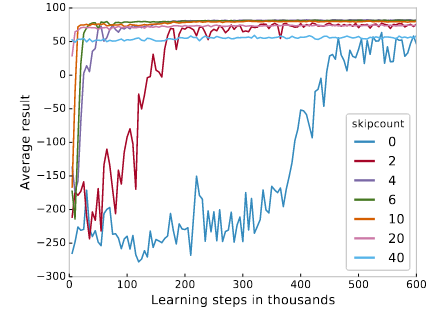
\includegraphics[scale=.8]{src/img/average-result-doom.png}
    \caption{Average Result per Steps - Doom Agent}
\end{figure}

\begin{figure}[H]
    \centering
    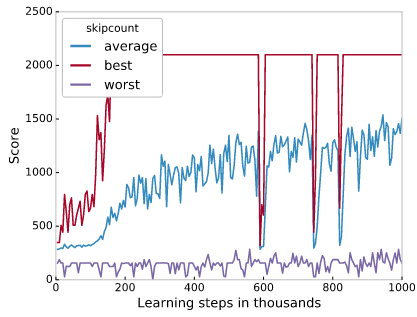
\includegraphics[scale=.8]{src/img/score-doom.png}
    \caption{Score per Steps - Doom Agent}
\end{figure}

\pagebreak

\section{Biomecânica}

\subsection{Ambiente}

O exemplo de \textit{environment} para esse caso de uso é o \textit{OpenSIM RL}\cite{osimrl}, uma biblioteca construída para simular algums movimentos mecânicos do corpo, como andar ou mover as mãos.

\subsection{Agente}

Um agente para esse ambiente tenta aprender alguma das funções fisiológicas regulares, como correr ou mexer os dedos, o espaço de observação é um vetor com os valores de tensão e força nos músculos, juntas e dados sobre velocidade e aceleração do corpo. As ações são também um vetor de 0's (zeros) e 1's (uns) para "liberar" ou "estressar" um músculo.

\subsection{Recompensas}

As recompensas variam a depender do ambiente escolhido, mas a recompensa para o mais popular, o \textit{L2RunEnvPermalink}, que visa criar um agente que aprenda a correr, tem a recompensa dada pela distância alcançada.

\subsection{Trabalhos correlatos}

A maioria dos trabalhos sobre esse ambiente foram expostos na \textit{NeurIPS}, uma das maiores conferências do mundo na área de aprendizado de máquina e neurociência, realizada anualmente até o ano de 2019 e após isso congelada até 2022 por conta da pandemia.

Os resultados são promissores e podem ser vistos na documentação nas referências, já que os resultados são vídeos ou animações do agente em ação.

\section{Minha escolha}

Meu método de escolha é baseado na praticidade do ambiente e para isso eu considero: \textit{setup} necessário para simular o ambiente e complexidade para receber o espaço de observação e enviar uma ação.

Dado isso, o ambiente do \textit{OpenSIM} foi eliminado, pois a maioria dos ambientes estão quebrados e tomariam muito tempo para serem configurados devido a um abandono de ambientes mais antigos por parte dos desenvolvedores, que priorizam os ambientes das próximas competições.

Portanto, pensando nas aplicações potenciais de cada agente, eu decidi seguir com o \textit{VizDoom}, por já possuir trabalhos acadêmicos na área, permitindo fazer um comparativo de desempenho.

\pagebreak
\printbibliography
\pagebreak

\end{document}
